\documentclass{article}

\usepackage{blindtext} % Package to generate dummy text throughout this template

\usepackage[sc]{mathpazo} % Use the Palatino font
\usepackage[T1]{fontenc} % Use 8-bit encoding that has 256 glyphs
\linespread{1.05} % Line spacing - Palatino needs more space between lines
\usepackage{microtype} % Slightly tweak font spacing for aesthetics

\usepackage[english]{babel} % Language hyphenation and typographical rules

\usepackage[hmarginratio=1:1,top=32mm,columnsep=20pt]{geometry} % Document margins
\usepackage[hang, small,labelfont=bf,up,textfont=it,up]{caption} % Custom captions under/above floats in tables or figures
\usepackage{booktabs} % Horizontal rules in tables

\usepackage{lettrine} % The lettrine is the first enlarged letter at the beginning of the text

\usepackage{enumitem} % Customized lists
\setlist[itemize]{noitemsep} % Make itemize lists more compact

\usepackage{abstract} % Allows abstract customization
\renewcommand{\abstractnamefont}{\normalfont\bfseries} % Set the "Abstract" text to bold
\renewcommand{\abstracttextfont}{\normalfont\small\itshape} % Set the abstract itself to small italic text

\usepackage{titlesec} % Allows customization of titles
\renewcommand\thesection{\Roman{section}} % Roman numerals for the sections
\renewcommand\thesubsection{\roman{subsection}} % roman numerals for subsections
\titleformat{\section}[block]{\large\scshape\centering}{\thesection.}{1em}{} % Change the look of the section titles
\titleformat{\subsection}[block]{\large}{\thesubsection.}{1em}{} % Change the look of the section titles

\usepackage{titling} % Customizing the title section

\usepackage{hyperref} % For hyperlinks in the PDF

\usepackage{logicpuzzle} % For drawing minesweeper configuration

\usepackage{float} % For locating figure

\usepackage{pifont}

%----------------------------------------------------------------------------------------
%	TITLE SECTION
%----------------------------------------------------------------------------------------

\setlength{\droptitle}{-4\baselineskip} % Move the title up

\pretitle{\begin{center}\Huge\bfseries} % Article title formatting
\posttitle{\end{center}} % Article title closing formatting
\title{The NP-Complete Problem: Minesweeper} % Article title
\author{%
\textsc{Liqiang Bao} \\[1ex] % Your name
\normalsize 201628008629002 \\
\normalsize University of Chinese Academy of Science \\ % Your institution
\normalsize \href{mailto:baoliqiang16@mails.ucas.ac.cn}{baoliqiang16@mails.ucas.ac.cn} % Your email address
%\and % Uncomment if 2 authors are required, duplicate these 4 lines if more
%\textsc{Jane Smith}\thanks{Corresponding author} \\[1ex] % Second author's name
%\normalsize University of Utah \\ % Second author's institution
%\normalsize \href{mailto:jane@smith.com}{jane@smith.com} % Second author's email address
}
\date{\today} % Leave empty to omit a date
\renewcommand{\maketitlehookd}{%
\begin{abstract}
\noindent Minesweeper has been one of my favourite computer games for many years. But few people know that this simple game could be related to one the most hard problems in the history. In this short report I will try to reveal this relation between them, and make a brief explanation why this game is too hard to solve. If we dive into the NPC classes, we'll find that the Minesweeper problem is just the tip of the iceburg. I hope that this report can be a magic mirror to the mysterious wonderland, for people who are interested or not interested, in the problems themselves or the prize.
\end{abstract}
}

%----------------------------------------------------------------------------------------

\begin{document}

% Print the title
\maketitle

%----------------------------------------------------------------------------------------
%	ARTICLE CONTENTS
%----------------------------------------------------------------------------------------

\section{Introduction}

As a short review of what the class has already been introduced to, we know that there exists a classification of problems in NP, problems referred to as NP Complete, that can be used to solve any other problem in NP provided there exists an algorithm that can solve the original problem. The concept of NP-completeness was introduced in 1971, though the term NP-complete was introduced later. At 1971 STOC conference, there was a fierce debate among the computer scientists about whether NP-complete problems could be solved in polynomial time on a deterministic Turing machine. John Hopcroft brought everyone at the conference to a consensus that the question of whether NP-complete problems are solvable in polynomial time should be put off to be solved at some later date, since nobody had any formal proofs for their claims one way or the other. This is known as the question of whether P=NP.

Nobody has yet been able to determine conclusively whether NP-complete problems are in fact solvable in polynomial time, making this one of the great unsolved problems of mathematics. There is a prize offering a US \$1 million reward to anyone who has a formal proof that P=NP or that P≠NP. The prize is one of seven now on offer from the newly founded Clay Mathematics Institute in Cambridge MA, set up by businessman Landon T. Clay to promote the growth and spread of mathematical knowledge, each bearing a million-buck price-tag.

\begin{figure}[H]
   \centering
   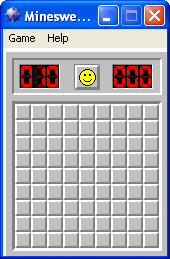
\includegraphics[scale=0.6]{images/minesweeper.png}
   \caption[]{Example of a Beginner-Level Minesweeper Board.}
   \label{fig_ms}
\end{figure}

Minesweeper comes with Microsoft's Windows operating system. In it, the player is presented with an initially blank grid. Underneath each square there may be a mine, and the object of the game is to locate all these mines without being blown up. You select a square to be revealed; if it is a mine you are blown up (and the game is over), but with luck, perhaps it isn't. In this second case, when the square is revealed you see a number from 0 to 8, which is the number of mines in the eight immediately neighbouring squares. 

It's not often you can win a million dollars by analysing a computer game, but by a curious conjunction of fate, there's a chance that you might. By cleverly constructing a reduction from \textit{Mineswpper Consistency Problem} to \textit{Circuit Satisfiability Problem}, Richard Kaye made a remarkable discovery, that the simple Minesweeper game is somehow a member of the NPC family and is very hard to solve by today's best computers. This conclusion sounds ridiculous, but you should keep in mind that you can't win the prize simply by winning the game. To win the prize, you should try to find a really slick method to actually answer question about whether a tile is a hidden mine. if you can decide this problem, which means, you can be 100\% sure to find all the mines without any hesitation, you win the prize. However, if you can also find a slick way to prove that there is no such a slick method, you win the prize too.

%------------------------------------------------

\section{Minesweeper Consistency Problem}

\begin{center}
  \begin{minesweeper}[rows=6,columns=6,scale=.8]
    \framepuzzle
    \setrow{6}{\ding{51},2,\ding{51}}
    \setrow{5}{\ding{51},\ding{51},\ding{51}}
    \setrow{4}{{},0,0,0,0,0}
    \setrow{3}{4,0,0,0,0,0}
    \setrow{2}{{},{},{},0,0,0}
    \setrow{1}{6,{},{},0,0,1}
  \end{minesweeper}
  \hspace{1.5cm}
  \begin{minesweeper}[rows=6,columns=6,scale=.8]
    \framepuzzle
    \setrow{6}{0,0,\ding{51},\ding{51},0,0}
    \setrow{5}{0,2,2,2,2,0}
    \setrow{4}{\ding{51},2,0,0,2,\ding{51}}
    \setrow{3}{\ding{51},2,0,0,2,\ding{51}}
    \setrow{2}{0,2,2,2,2,0}
    \setrow{1}{0,0,\ding{51},\ding{51},0,0}
  \end{minesweeper}
\end{center}

The \textit{Minesweeper Consistency Problem} is not to find the mines, but to determine whether a given state of what purports to be a Minesweeper game is or is not logically consistent. For example, if during the state of play you encountered the left configuration above, you would know that the programmer had make a mistake: there is no allocation of mines consistent with information shown. But if you encountered the right one above, you will agree that this configuration is totally right. That is, The \textit{Minesweeper Consistency Problem} is to determine if a given configuration is consistent. 

For the reason of simplicity, we will refer \textit{Minesweeper problem} as \textit{Minesweeper Consistency Problem}. As discussed above, this is a typical yes/no problem, and if we could solve this problem efficiently with a computer, we would have an excellent method for playing the game. To determine if a square is safe, we could mark the current square in question with a mine, and feed this mark into the computer together with the configuration. If the computer says that this pattern is inconsistent, then there is no mine at the square in question and it is safe to reveal it, otherwise there may be a mine.

%------------------------------------------------

\section{Minesweeper is NPC-complete}

We already know that \textit{CIRCUIT-SAT} is NP-complete, to prove that Minesweeper is NP-complete, we must show that Minesweeper is in NP and that any language A in NP is reducible to Minesweeper. The first is obvious, for to determine if an incomplete configuration is consistent, it suffices to guess the positions of the mines and then verify that these mines produce the numbers seen. To do the second we reduce \textit{Minesweeper problem} to \textit{CIRCUIT-SAT problem} in polynomial time.

We can use the fact that mines’ locations and information on one side of the grid can influence information on another side of the grid to our advantage since, essentially, this is what circuits do. Examine the configuration in Figure \ref{fig_wire}, where the letters $x$ and $x'$ label unrevealed squares which may or may not contain mines. Fundamentally, wires are a way to transfer the same value from one location to another. In \textit{Minesweeper}, We can regard this configuration as a wire carrying a value which is TRUE or FALSE depending on whether the $x$ or $x'$ have the mines.

\begin{figure}[H]
  \centering
  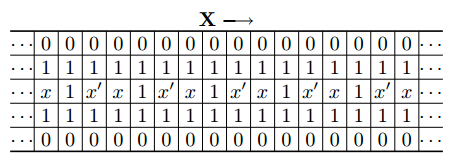
\includegraphics[scale=.9]{images/wire.png}
  \caption{A wire}
  \label{fig_bend}
\end{figure}

We will need to be able to bend wires, and to split them. Figure \ref{fig_bend} and \ref{fig_split} shows how to do it. In those configurations, the squares marked $\star$ have mines in them. Figure \ref{fig_bend}(a) is a simple $90\deg$ bend in the wire. Figure \ref{fig_split}(b) shows how a wire can be terminated. Figure \ref{fig_split} shows a way of "splitting" a wire. Any of these wires can be terminated by a piece as in Figure \ref{fig_bend}(b) and the splitter can be combined with bends and further splitters, to make splitters with any number of outputs.

\begin{figure}[H]
  \centering
  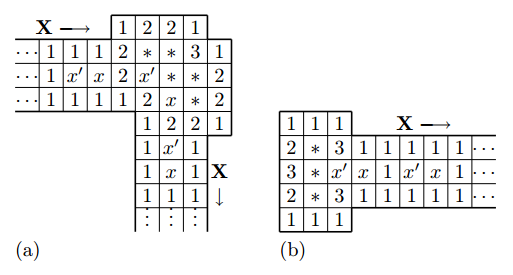
\includegraphics[scale=.9]{images/bend.png}
  \caption{(a) A bent wire. (b) A terminated wire.}
  \label{fig_wire}
\end{figure}

\begin{figure}[H]
  \centering
  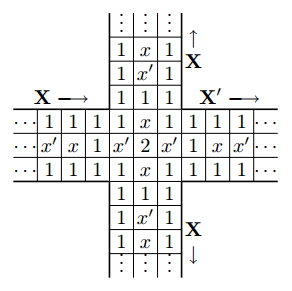
\includegraphics[scale=.9]{images/split.png}
  \caption{A three-way splitter.}
  \label{fig_split}
\end{figure}

We are now familiar with the simplest form of information transfer in \textit{Minesweeper}, but if we are to prove it as NP Complete, we will expect \textit{Minesweeper} to be able to behave in much more versatile ways than simply retaining information about a square’s truth value. Remember that circuits have a series of logic gates (AND, OR, NOT, XOR, etc) that each take in two boolean inputs to output one boolean value. Fortunately, this has been done. In fact, \textit{Minesweeper} has all of the necessary arrangements for grids that can perform in the same way that these logic gates do.

NOT gate is a very important device for logic circuits, in Figure \ref{fig_not} we show how to construct a NOT gate. Since we defined truth/falsity in a wire relative to the position of the centre is in the wire, we may find a problem when we want to combine two or more signals if they are not aligned correctly. In Figure \ref{fig_pc}, by combining two NOT gates, we can construct a Phase Changer which can handle the alignment problem.

\begin{figure}[H]
  \centering
  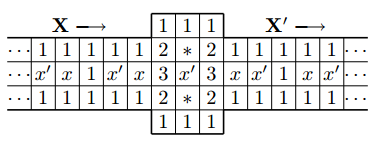
\includegraphics[scale=.9]{images/not.png}
  \caption{A NOT gate.}
  \label{fig_not}
\end{figure}

\begin{figure}[H]
  \centering
  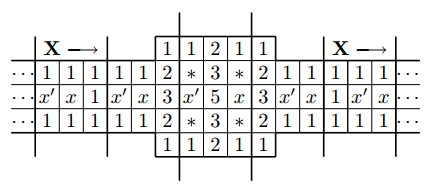
\includegraphics[scale=.9]{images/phase-changer.png}
  \caption{A phase-changer made from two not gates.}
  \label{fig_pc}
\end{figure}

In order to mimic arbitrary boolean circuits we need to have more complex AND, OR, XOR gates, and so on. In Figure \ref{fig_and}, The AND gate has two internal wires, $R$ and $S$, which are aligned and looped back to a splitter at the output $T$ via a pair of devices labelled $a_1,a_2,a_3$ and $b_1,b_2,b_3$. To understand how it works here, we first see what happens if we set the output to TRUE, i.e., if the $t$s are mines and the $t'$s are not. In this case, from the 3 above and below $a_3$, we have that $a_2$ and $a_3$ must be mines, so $a_1$ is clear, and $s$ is a mine. Similarly $r$ is a mine. Thus the central 4 already sees four mines--$s$, $t$, $r$, and the *--so $u'$, $v'$ are both clear and the inputs $U$, $V$ are both true. This shows that if $t$ is a mine, all the other unknown squares are determined, and it is straightforward to check that these
values are consistent with the data given. Thus we can prove the correctness of this AND gate by considering other cases.

\begin{figure}[H]
  \centering
  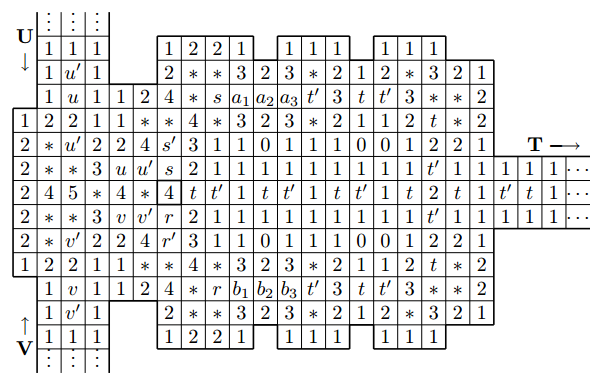
\includegraphics[scale=.9]{images/and.png}
  \caption{An AND gate.}
  \label{fig_and}
\end{figure}

In the same way as explained above, we have OR gate and XOR gate in Figure \ref{fig_or} and Figure \ref{fig_xor}.

\begin{figure}[H]
  \centering
  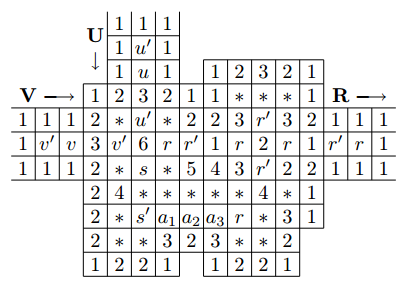
\includegraphics[scale=.9]{images/or.png}
  \caption{A OR gate.}
  \label{fig_or}
\end{figure}

\begin{figure}[H]
  \centering
  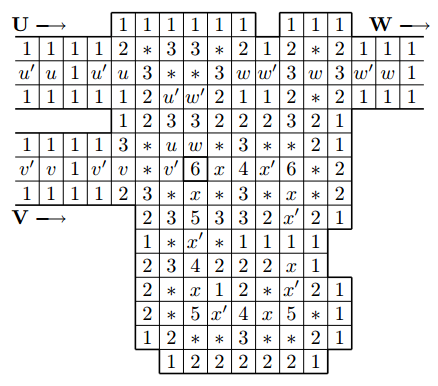
\includegraphics[scale=.9]{images/xor.png}
  \caption{A XOR gate.}
  \label{fig_xor}
\end{figure}

Now since we have all the gates we need, it becomes easier to simulate or construct any boolean circuit grid out of the ones already done. If we can determine the \textit{Minesweeper problem} in polynomial, we can also determine a boolean assignment to the variables in \textit{CIRCUIT-SAT problem}. Therefore, both problems are NP-complete.

%------------------------------------------------

\section{A simpler Proof}

Now we formally show that \textit{Minesweeper} is NP-complete in a simpler way, completing the alternative proof of the Cook-Levin theorem. \\
\\
\textbf{CLAIM:} \textit{Minesweeper} is NP Complete.
\\
\textbf{PROOF:}
\begin{itemize}
  \item \textbf{\textit{Minesweeper} is in NP} \\
  We begin by attempting to show that \textit{Minesweeper} is in NP. Suppose we are given a potential solution to an arbitrary Minesweeper grid (in other words, a completely revealed board that has no hidden squares). In order to verify that the solution is consistent, a computer algorithm would step through the grid, one square at a time, verifying that every number has exactly that number’s indicated value of mines as neighbors. Each square has a maximum of 8 adjacent squares to check, so given a Minesweeper grid with $n$ squares, the runtime will be at most $8t\times n$ (where $t$ is the amount of time necessary to check one square’s adjacent partner). Since this algorithm clearly runs in polynomial time, the \textit{Minesweeper} problem is in NP.
  \item \textbf{\textit{Minesweeper} is in NP hard} \\
  The fact that \textit{Minesweeper} is in NP is not enough; we must also prove that this problem is NP Hard. Assume we are given an arbitrary boolean circuit that inputs the variables $x_1,x_2,\cdots,x_n$ and outputs the value $y$. This circuit will have a series of AND, OR, and NOT configurations, which eventually assigns either true or false to $y$ depending on the initial values of our variables. We want an initial boolean value assignment to each variable that will output the value true for $y$ (this, by definition, is our \textit{CIRCUIT-SAT problem}). Since we are able to construct wires, ANDs, ORs, and NOT functions in Minesweeper, we can build a corresponding Minesweeper grid to our circuit. At the "end" or our constructed Minesweeper grid, we assign a mine to the value of $y$ (essentially forcing this value to be true). Assuming we have an algorithm that determines Minesweeper consistency in polynomial time, we can determine a boolean assignment to our initial variables (mine or no mine) that will remain consistent with our assignment of a mine on $y$. Therefore, circuit satisfiability, in this way, can be determined using Minesweeper Consistency, provided we had an algorithm that runs in polynomial time to check this. Because we know that circuit satisfiability is NP Hard (it can be used to solve any problem in NP), Minesweeper Consistency must therefore be NP Hard as well.
  \item \textbf{\textit{Minesweeper} is in NP-complete} \\
  Since Minesweeper Consistency has been shown to be in NP and is NP Hard, by definition, it is NP-Complete.
\end{itemize}

%----------------------------------------------------------------------------------------
%	REFERENCE LIST
%----------------------------------------------------------------------------------------

%\clearpage
\section{Sources}

Kaye, Richard. "Minesweeper is NP-complete." The Mathematical Intelligencer 22.2 (2000): 9-15. \\
\\
Cook, Stephen A. "The complexity of theorem-proving procedures." Proceedings of the third annual ACM symposium on Theory of computing. ACM, 1971. \\
\\
Stewert, Ian. Million Dollar Minesweeper. \\
\url{http://www.minesweeper.info/articles/MillionDollarMinesweeper.pdf} \\
\\
Kaye, Richard. Some Minesweeper Configurations. \\
\url{http://web.mat.bham.ac.uk/R.W.Kaye/minesw/minesw.pdf} \\

%----------------------------------------------------------------------------------------

\end{document}
